
\begin{figure}
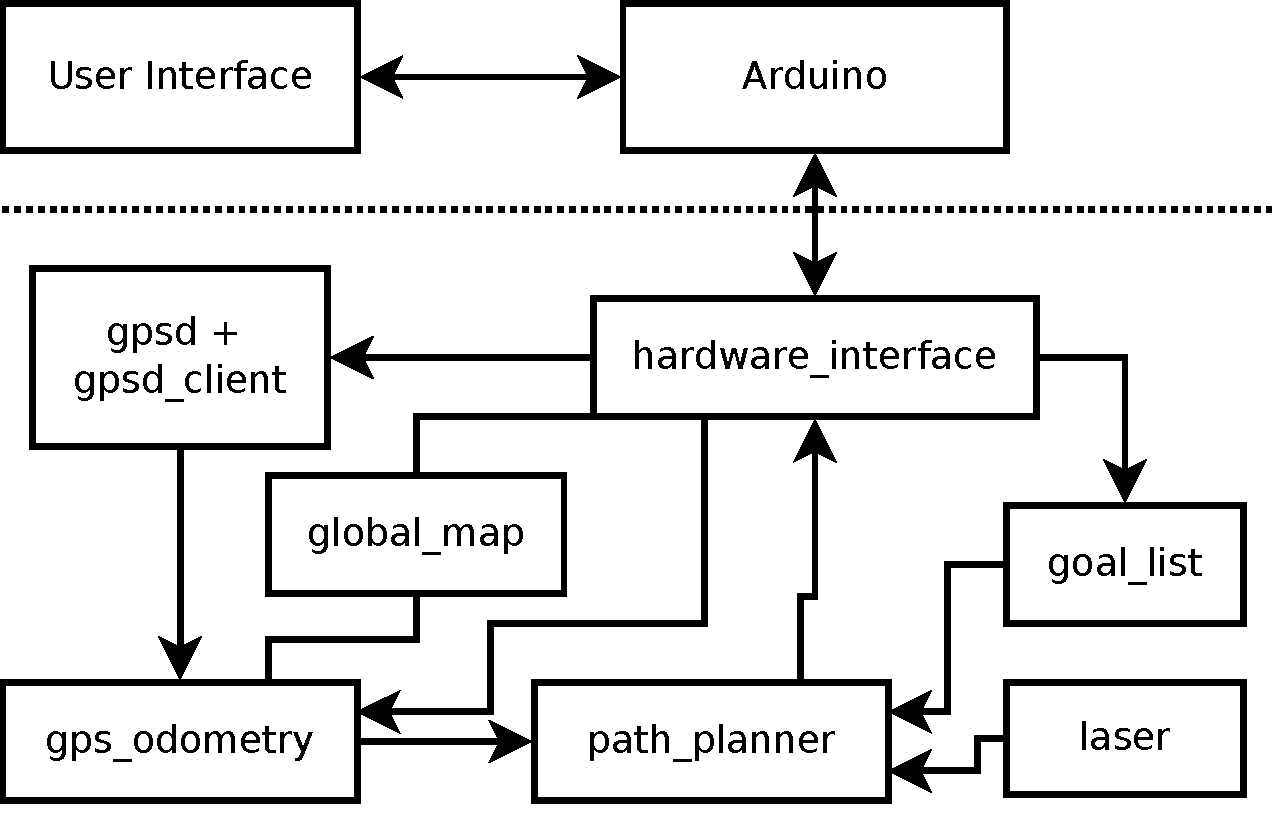
\includegraphics[width=1\textwidth]{software_flow}
\caption{ROS Node and Dataflow Diagram}
\end{figure}

The primary computer runs Gentoo, a Linux distribution, and runs the ROS software package to support the high-level behaviors. Each behavior or part of the system is implemented as a separate ROS node, and communicates with other nodes through messages or service calls.

The \texttt{hardware\_interface} node is responsible for translating data from the Arduino into ROS messages, and for translating some ROS messages into control and status data to be sent to the Arduino. 

The \texttt{hardware\_interface} node recieves odometry, bump sensor, battery level, GPS, and compass data from the Arduino. It translates the odometry data into odometry messages, using a kinematic model of the robot to translate encoder counts and wheel movements into position change in x, y, and heading. It translates the compass data (really an x-y magnetometer) into a heading from north, and publishes that angle in a compass message. It takes the GPS data, as NMEA strings, and sends it to an instance of gpsd\cite{gpsd}, which parses the data, and publishes it, to be read by the \texttt{gpsd\_client} node, which publishes the resulting data as GPSFix messages. It records the battey level data into a log file, for later analysis; eventually, this data will be used to build a model to predict remaining battery capacity. It ignores the bump sensor data. The \texttt{hardware\_interface} node also receives a list of gps coordinates that is forwarded through the Arduino from the user interface, and publishes this as a GoalList message.

The \texttt{hardware\_interface} node recieves command messages as speed and steering commands, and transmits them to the Arduino. It also recieves position estimate messages, translates them into GPS coordinates, and transmits them to the Arduino, to be forwarded to the user interface.

The \texttt{global\_map} node is responsible for storing the map, and for the mapping of GPS coordinates to map coordinates. It uses a transverse mercator projection to map latitude/longitude coordinates onto a square grid. It chooses the nearest longitude line, to the nearest degree, to use as the local meridian for the projection. This makes it easy to choose a meridian based on the current position, it allows GPS coordinates to be mapped onto a square grid, and it minimizes the distortion when translating from one coordinate system to the other. The \texttt{global\_map} node provides a pair of ROS Services that map GPS coordinates to row/column addresses in the map, and from row/column addresses back to GPS coordinates.

The \texttt{goal\_list} node is responsible for maintaining the list of goals from the user, and for tracking which goal is the current goal. It receives new lists of goals from the \texttt{hardware\_interface}, and the current position of the robot, and publishes the current goal. It considers a goal to be reached when it is within a pre-configured distance, and moves on to the next goal.

The \texttt{gps\_odometry} node is responsible for performing Kalman filtering to fuse GPS, compass and odometry data to produce a more accurate position estimate. It's implemented as two kalman filters; one for row/column position in map coordinates, and separate filter for heading. This was possible because there is no correlation between the robot's heading and its position; it allows for simpler update steps and smaller covariance matrices. Updates are done whenever new data arrives, based on the type of the data. Odometry is treated as a prediction update, while compass and GPS data is treated as measurement updates.

The \texttt{path\_planner} node is responsible for directing the robot from its current position to the current goal position while avoiding obstacles. It receives the position of the robot, the current goal, and laser scan data, and publishes steering and speed commands to the \texttt{hardware\_interface}. It is implemented as reactive goal follower with obstacle avoidance; it computes the desired heading to the goal based on the robot's position, then checks to see that this heading is obstacle-free, based on the most recent scan from the laser. If it isn't, it searches headings to either side of the desired heading until it finds one that is obstacle free. It uses this heading to compute the desired change in heading, and uses that to proportionally control the steering. It sets a constant forward speed.

The laser node is a stock ROS node (\texttt{hokuyo\_node}) that reads data from the laser over USB, and publishes it as a ROS message.
